\documentclass[10pt,aspectratio=169,handout]{beamer}
\usefonttheme[onlymath]{serif}


\usetheme[progressbar=frametitle]{metropolis}
\usepackage{appendixnumberbeamer}

\usepackage{booktabs}
\usepackage{bbm}
\usepackage[scale=2]{ccicons}
\usepackage{macros}
\usepackage{natbib}
\bibliographystyle{aer}
% \usepackage{euler}
\usepackage{sourcesanspro}

\setmonofont{inconsolata}

% \usepackage{lmodern}
\usepackage{pgfplots}
\usepgfplotslibrary{dateplot}

\usepackage{xspace}
\usepackage{fontspec}
\usepackage{mathspec}
\usepackage{adjustbox}
\usepackage{cancel}
\usepackage{verbatim}

\usepackage{tikz}
\usetikzlibrary{decorations.pathmorphing}
\newcommand\Wasserman{\tikz[baseline=-0.8ex]{\draw[line width=0.07em,decorate,decoration={coil,segment
length=0.45em,amplitude=0.8ex}] (0,0) -- (2em,0);}}


\metroset{block=fill}
\theoremstyle{definition}
\newtheorem{thm}{Theorem}

\newtheorem{prop}{Proposition}
\newtheorem{defn}{Definition}
\newtheorem{cor}{Corollary}

\newtheorem{ex}{Example}

% \newcommand{\E}{\mathbb{E}}

\newcommand{\themename}{\textbf{\textsc{metropolis}}\xspace}


% \newfontfamily\bodyfont[]{Source Code Pro}
% \newfontfamily\thinfont[]{Source Code Pro ExtraLight}
% \newfontfamily\headingfont[]{Source Code Pro Black}
% % %
% \defaultfontfeatures{Mapping=tex-text}
% \setmainfont[Mapping=tex-text, Color=textcolor]{Source Code Pro Light}


\definecolor{maroon}{RGB}{73,10,61}
\definecolor{orange}{RGB}{233,127,2}
\definecolor{yellow}{RGB}{248,202,0}
\definecolor{green}{RGB}{138,155,15}


\definecolor{crimson}{RGB}{192,41,66}
\definecolor{purple}{RGB}{84,36,55}
\definecolor{pastel}{RGB}{236,208,120}
\definecolor{aqua}{RGB}{83,119,122}
\definecolor{brick}{RGB}{217,91,67}

\makeatletter
\g@addto@macro\small{
\setlength\abovedisplayskip{4pt}
\setlength\belowdisplayskip{4pt}
\setlength\abovedisplayshortskip{4pt}
\setlength\belowdisplayshortskip{4pt}
}
\makeatother


\hypersetup{
  colorlinks=true,
  linkcolor=,
  citecolor=maroon
}

% \setsansfont[BoldFont={Source Sans Pro Semibold}]{sourcesanspro}

\setmathfont{Latin Modern Math}
\setbeamercolor{alerted text}{bg=brick, fg=crimson}

\setbeamercolor{frametitle}{bg=crimson, fg=white}
\setbeamercolor{progress bar}{bg=pastel, fg=brick}
\setbeamercolor{title separator}{bg=crimson}

% \usepackage[citecolor=brick]{hyperref}
\newcommand{\light}[1]{\textcolor{gray}{#1}}

\title{
Semiparametric theory}
\subtitle{}
\date{\today}
\author{Jiafeng Chen}
\institute{Econometrics Reading Group}
% \titlegraphic{\hfill\includegraphics[height=1.5cm]{logo.pdf}}

\begin{document}

\maketitle

\begin{frame}{}
\hyperlink{sec:applied}{\beamerbutton{applied talk}}
\end{frame}

\section{A tour of \emph{Semiparametric Theory and Missing Data}
\footnote{with a little of Ed Kennedy's tutorial and van der Vaart
mixed in}}

\begin{frame}{Semiparametric models}
  Observe data $Z_1,\ldots, Z_n \iid P_0$. $P_0$ belongs to a set of
  distributions
  $\mathcal P = \{P_{\beta,\eta}\}$. The model $\mathcal P$ is 
  \alert{semiparametric}  if, generally, $\beta$ is finite dimensional and
  $\eta$ is infinite dimensional.
  
  \begin{ex}
    Suppose $\beta = \E[Z]$ is the parameter of interest. If $\mathcal P =
    \{\Norm(\beta,1) : \beta \in \R\},$ the model is parametric. If
    $\mathcal P = \{P: \E_P[Z^2] < \infty\}$ contains all one dimensional
    distributions with finite second moment, then the model is
    semiparametric. In this case, we can treat the nuisance parameter as
    $\eta = \mathcal L(Z - \E[Z])$.
  \end{ex}
\end{frame}

\begin{frame}{Influence functions, RAL estimators}
  Assume for now that we have a finite-dimensional model $Z_1,\ldots, Z_n
  \iid P_\theta, \theta = (\beta,
  \eta)$, $\beta \in \R^q, \eta \in \R^r$. Most ``reasonable'' estimators
  $\hat \beta_n$
  are \alert{asymptotically linear}: \[
  \sqrt{n}(\hat\beta_n - \beta_0) = \frac{1}{\sqrt{n}} \sum_{i=1}^n \varphi
  (Z_i, \theta_0)+ o_{P_{\theta_0}}(1)
  \]
  The function $\varphi(\cdot) = \varphi(\cdot, \theta_0)$ is called the
  \alert{influence function} of $\hat \beta_n$. 
  \begin{prop}
    If $\hat\beta_n$ is asymptotically linear, its influence function is
    a.s. unique.
  \end{prop}
  
\end{frame}

\begin{frame}{Influence functions, RAL estimators}
    \begin{defn}[Regular estimators]
    Consider the \alert{local} DGP $P_n = P_{\theta_n}$ indexed by the
    drifting parameter $\theta_n = \theta_0 + h/\sqrt{n}$. Consider $Z_
    {1n},\ldots, Z_{nn} \iid P_{\theta_n}$. An estimator is 
    \alert{regular} if the limiting distribution
     $\sqrt{n}(\hat\beta_n - \beta_n) \overset{\theta_n}{\leadsto} L_
    {\theta_0}$ doesn't depend on $h$.
  \end{defn}
  
  \begin{ex}
    $Z_1,\ldots, Z_n \sim \Norm(\beta,1)$. The sample mean $\hat\beta_n =
    \frac{1}{n}\sum_i Z_i$ is RAL (regular and asymptotically linear) with
    influence function $\varphi(Z,
    \beta) = Z-\beta$
  \end{ex}
\end{frame}

\begin{frame}{Structure of influence functions (parametric model)}
\small
  Let $\theta \in \R^p$ be the parameter and let's say we are interested in
  $\beta
  (\theta) \in \R^q$ [slightly more general than $\theta = (\beta, \eta)$].
  
  \alert{Pathwise derivative representation of the influence function}
  \begin{thm}[Tsiatis Theorem 3.2; Newey (1994) expression (2.2); Newey 
    (1990) Theorem 2.2]
    Let $\Gamma^{q\times p}(\theta) = \diff{\beta}{\theta'}$.  
    \light{Assume $\Gamma$ exists, full rank, continuous in a neighborhood
    of $\theta_0$.} Let $\hat \beta_n$ be AL with influence function
    $\varphi(Z)$ \light{s.t. $\E_\theta[\varphi'\varphi]$ exists,
    continuous in $\theta$ in a neighborhood of $\theta_0$.} 
    Let $S_\theta(z,\theta) = \diff{}{\theta} p(z,\theta)$ be the score.
    Then if
    $\hat\beta_n$ is regular, \[
    \E[\varphi(Z) S_\theta'(Z,\theta_0)] = \Gamma(\theta_0)
    \]
  \end{thm}
  
  \begin{cor}
    If $\theta = (\beta, \eta)$, let $S_\theta = [S_\beta, S_\eta]$, then 
    \begin{align*}
    \E[\varphi(Z)S_\beta'] &= I_q \\ \E[\varphi(Z)S_\eta'] &= 0^{q\times r}
    \end{align*}
  \end{cor}
  
\end{frame}

\begin{frame}{Structure of influence functions (parametric model)}
\small
    \begin{thm}
    Let $\Gamma^{q\times p}(\theta) = \diff{\beta}{\theta'}$.  
    Let $\hat \beta_n$ be AL with influence function
    $\varphi(Z)$.
    Let $S_\theta(z,\theta) = \diff{}{\theta} p(z,\theta)$ be the score.
    Then if
    $\hat\beta_n$ is regular, \[
    \E[\varphi(Z) S_\theta'(Z,\theta_0)] = \Gamma(\theta_0)
    \]
  \end{thm}
  
  \begin{proof}[Sketch]
    Consider RAL $\hat\beta_n$. Under local sequence $\theta_0 = \theta_n
    + h/\sqrt{n}$, \begin{align*}
         \overbrace{\sqrt{n} (\hat\beta_n
        - \beta(\theta_n))}^{\Norm(0, \E_{\theta_0}[\varphi\varphi'])} &= \sqrt{n}(\hat \beta_n
    - \beta(\theta_0)) - \sqrt{n}(\beta(\theta_n) - \beta(\theta_0)) \\ 
    &\simeq_{\theta_n} \underbrace{ \frac{1}{\sqrt{n}}\sum_i \bk{\varphi
    (Z,\theta_0) -
    \E_
            {\theta_n}[\varphi(Z, \theta_0)]}}_{\Norm(0, \E_{\theta_0}
            [\varphi\varphi'])} + \sqrt{n}\E_{\theta_n}[\varphi
        (Z,\theta_0)] - \sqrt{n}(\beta(\theta_n) - \beta(\theta_0))
    \end{align*}
    Equate the latter two terms to zero. Differentiate w.r.t. $\theta$ to
    linearize. Get $\E[\varphi S'_\theta]$ from the first, $\Gamma$ from
    the second.
    \end{proof}
\end{frame}

\begin{frame}{Tangent spaces, Geometry of IF}
\small
  Let $\theta = [\beta,\eta]$.

  The score $S_{\theta}(Z, \theta_0)$ (which is mean zero $\E_{\theta_0} 
  [S_\theta(Z,\theta_0)] = 0$). Consider $\mathcal H$ the \alert{Hilbert
  space}
  formed by all $q$-dimensional $P_0$-mean-zero-finite-variance functions,
  equipped
  with the covariance inner product.
  
  \begin{defn}
    Let the \alert{tangent space} be $\mathcal T = \{BS_\theta(Z, \theta_0) : B\in \R^
    {q\times p}\} \subset \mathcal H$. Let the \alert{nuisance tangent
    space} be $\Lambda = \{BS_\eta(Z, \theta_0) : B \in \R^{q\times r}\}
    \subset \mathcal T \subset \mathcal H$. 
  \end{defn}
  
  Note that an influence function $\varphi$ necessarily has \alert{$\varphi
  \perp
    \Lambda$}.
    
    \begin{thm}[Converse to Theorem 3.2]
      Let $\varphi(Z)$ be such that $\E[\varphi S_\beta'] = I, \E[\varphi
      S_\eta'] = 0$. The moment condition $m(Z,\beta,\eta) = \varphi(Z) -
      \E_{\beta,\eta}[\varphi(Z)]$ defines $\hat\beta_n$ that is RAL with
      influence function $\varphi(Z)$ so long as $\hat\eta_n$ is $
      \sqrt{n}$-consistent.
    \end{thm}
    Now we can talk about influence functions \alert{without} talking about
    RAL estimators. (This is often confusing!)
\end{frame}

\begin{frame}{Geometry of IF}
\small
  \begin{thm}
    The set of all influence functions is the \alert{linear variety} $
    \varphi(Z) + \mathcal T^\perp = \{\varphi(Z) + \phi(Z) : \phi \in
    \mathcal T^\perp\}
    $
    where $\varphi(Z)$ is \alert{any} influence function.
  \end{thm}
  
  \begin{defn}
    The variance-minimizing influence function (\alert{efficient
    influence function}) is the projection of any influence function onto
    the tangent space \[\varphi_{\text{eff}}(Z) = \Pi( \varphi(Z) |
    \mathcal
    T) = \Gamma(\theta_0) I^{-1}(\theta_0) S_\theta(Z,\theta_0) 
    \overset{\text{subvec}}{=} \E[\varphi S_\theta']\E[S_\theta
    S_\theta']^{-1} S_\theta = \mathrm{Cov} \cdot \mathrm{Var}^{-1}
    S_\theta.\]
    
    The \alert{efficient score} is the residual of the score after
    projecting onto the \alert{nuisance tangent space} \[
    S_{\text{eff}}(Z,\theta_0) = \Pi(S_\beta | \Lambda^{\perp}) = S_\beta -
    \E[S_\beta S_\eta'] \E[S_\eta S_\eta']^{-1} S_\eta
    \]
    
    We also have $\varphi_{\text{eff}} = \E[S_{\text{eff}}S_{\text{eff}}']^
    {-1}S_{\text{eff}}$ under the subvector $\theta = [\beta, \eta]$
  \end{defn}
\end{frame}

\begin{frame}{Attempt at visualizing tangent spaces and influence
functions}
  \begin{figure}[tb]
    \centering
    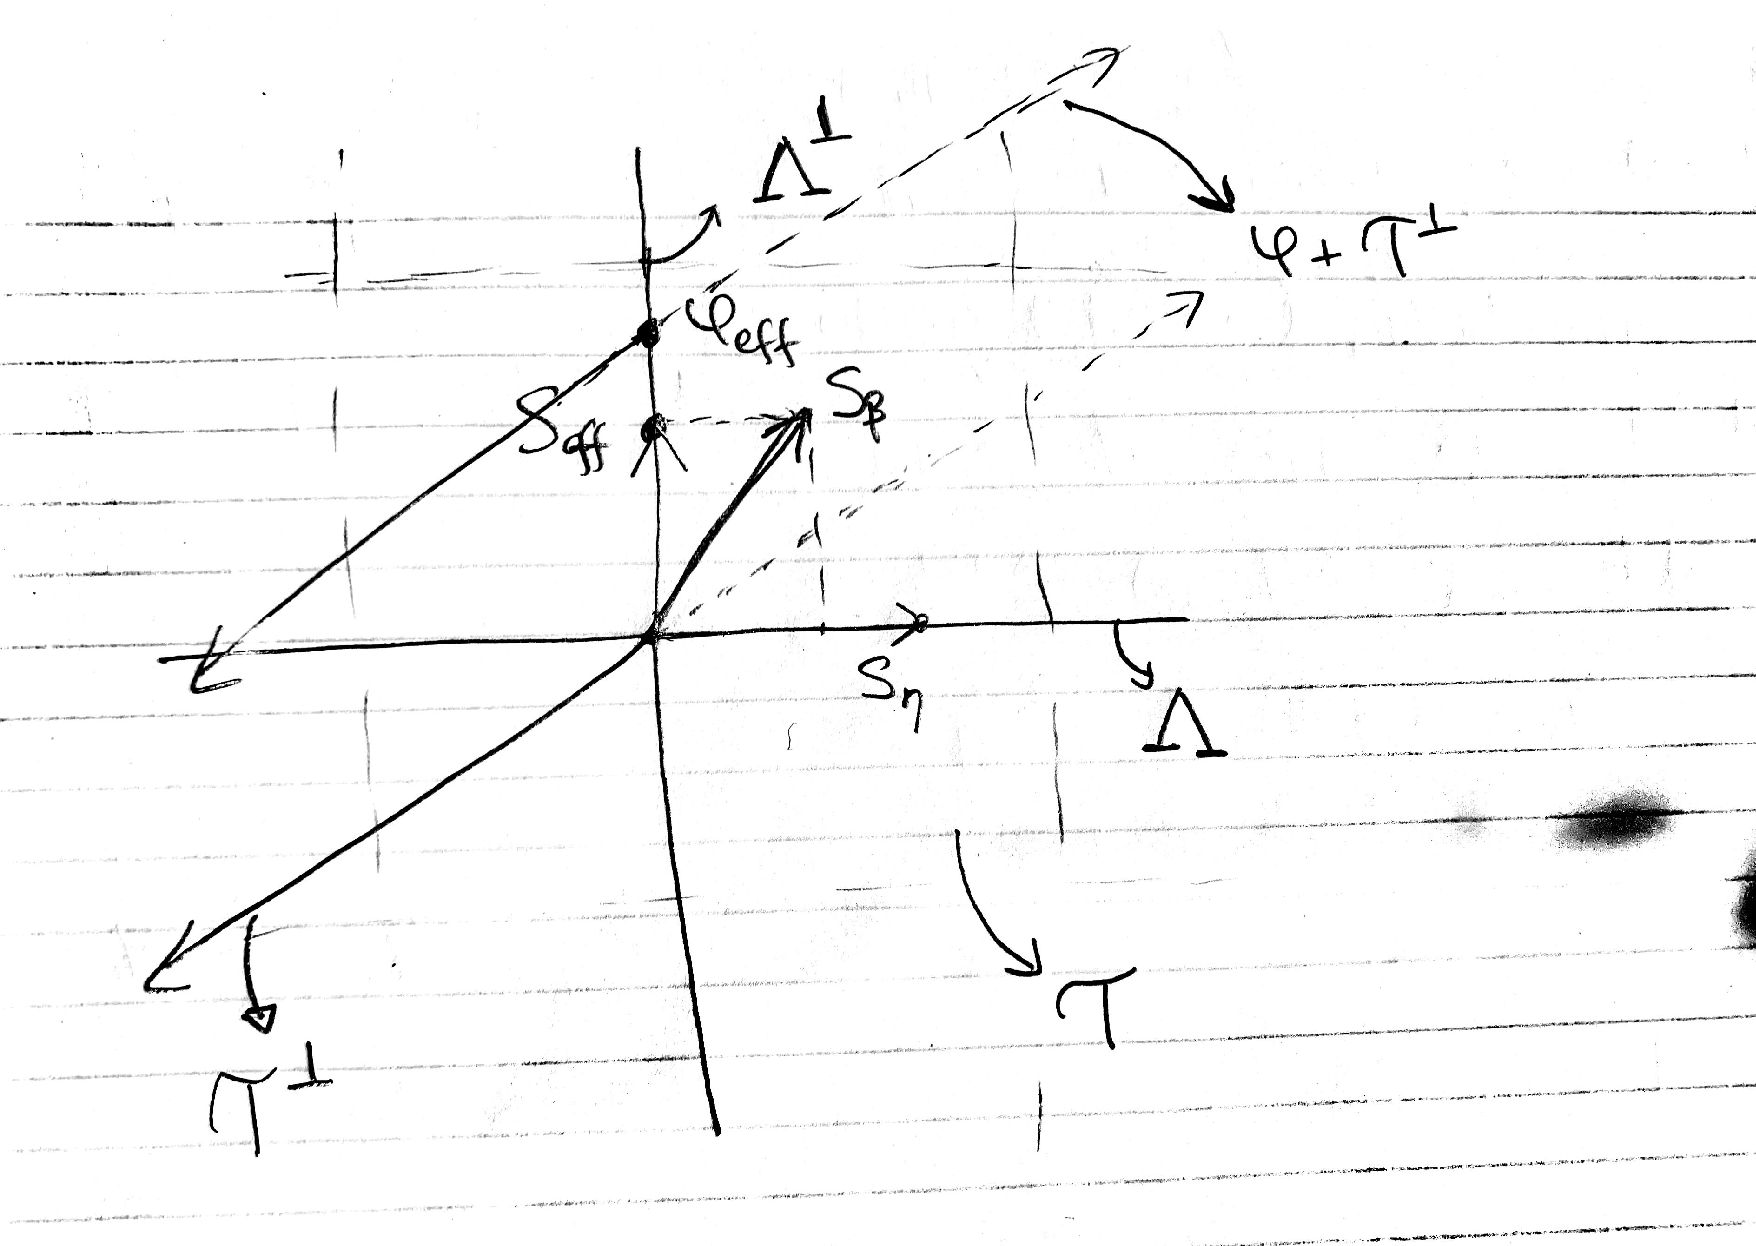
\includegraphics[height=0.8\textheight]{viz.pdf}
    \label{fig:figure1}
  \end{figure}
\end{frame}

\begin{frame}{Attempt at visualizing tangent spaces and influence
functions}
  \begin{figure}[tb]
    \centering
    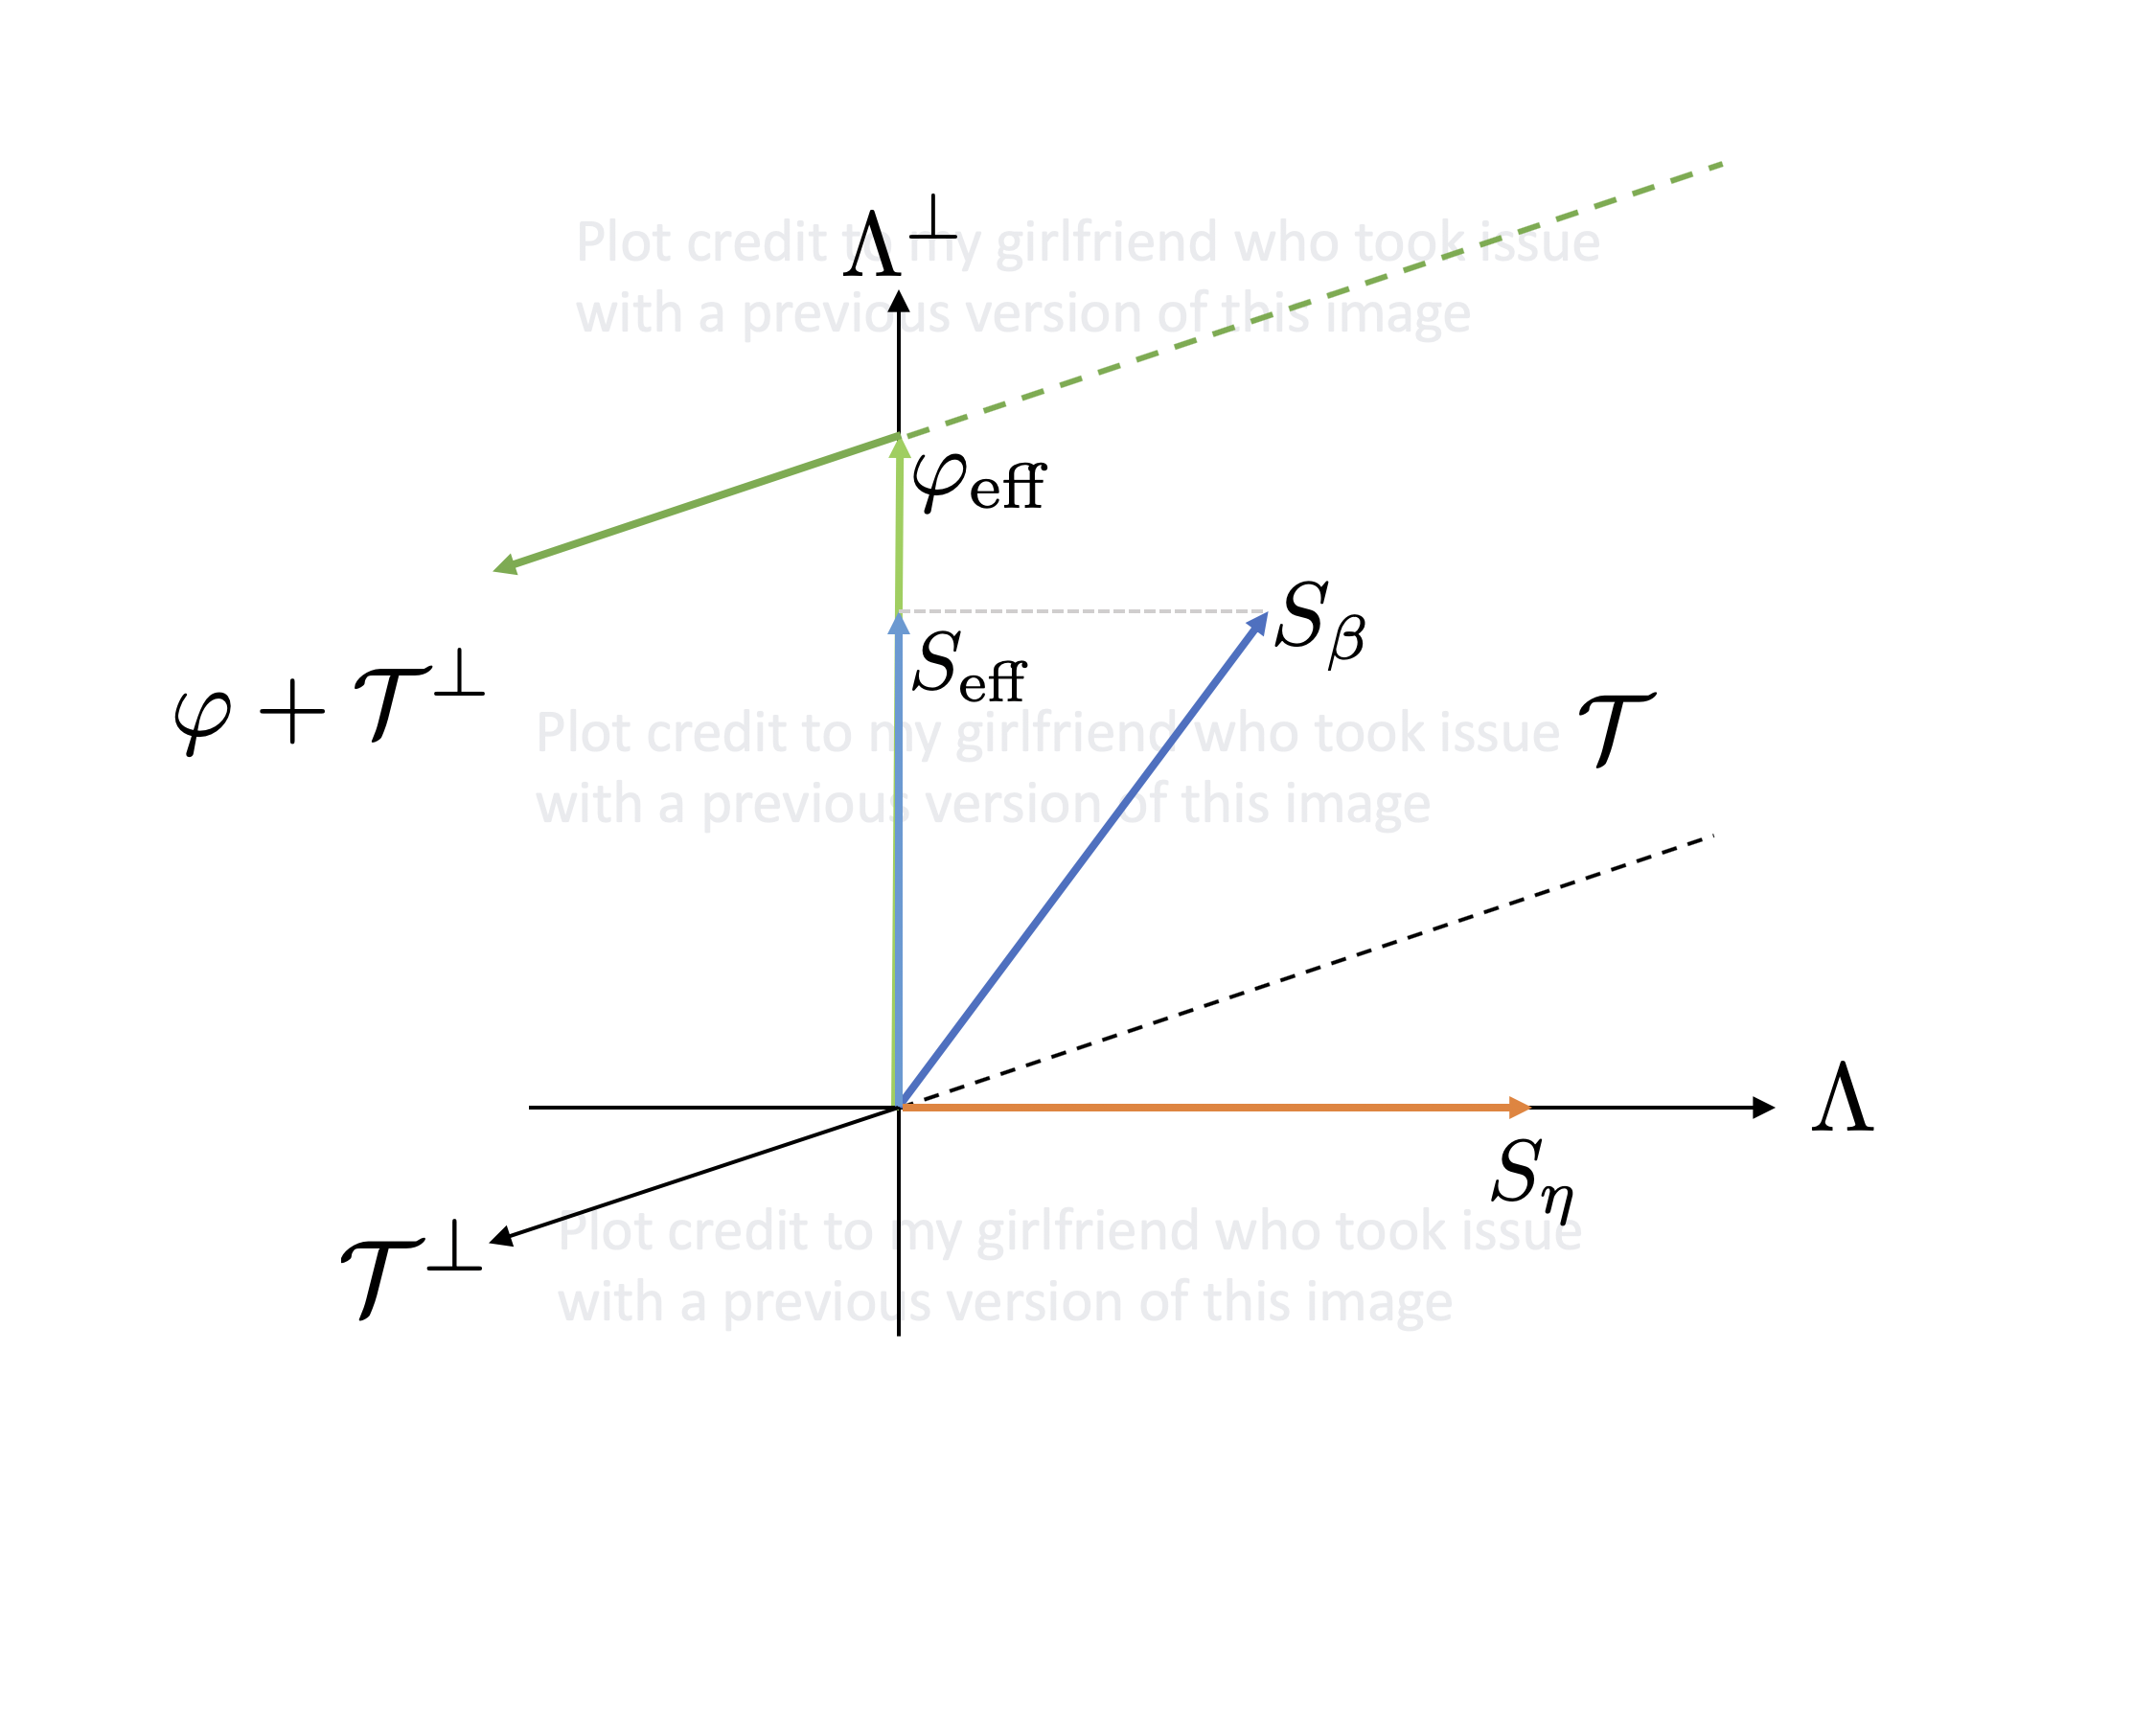
\includegraphics[height=0.9\textheight]{viz2.png}
    \label{fig:figure1}
  \end{figure}
\end{frame}


\begin{frame}{Example}
\begin{ex}[Making sure MLEs make sense]
    Consider the MLE in $\theta = (\beta, \eta).$ It is known to be
    efficient. The efficient variance is \[
    V^* = \E[S_\text{eff} S_\text{eff}']^{-1} = \E[\varphi_
    \text{eff}\varphi_\text{eff}'] = [I_\theta^{-1}]_{\beta}
    \]
    
    We can calculate the top-left of $I_\theta^{-1}$: \[
    V^* = (I_{\beta\beta} - I_{\beta\eta}I_{\eta\eta}^{-1} I_{\beta\eta}')^
    {-1}.
    \]
    Efficient score is \[
    S_{\text{eff}}= S_\beta - I_{\beta\eta} I_{\eta\eta}^{-1} S_\eta
    \]
    and so $\E[S_\text{eff} S_\text{eff}'] = (I_{\beta\beta} - 2 I_
    {\beta\eta}I_{\eta\eta}^{-1} I_{\eta\beta} + I_{\beta\eta} I_
    {\eta\eta}^{-1} I_{\eta\eta} I_{\eta\eta}^{-1} I_{\eta\beta})$
  \end{ex} 
\end{frame}

\begin{frame}{Summary for parametric models}
$\theta = [\beta,\eta]$
  \begin{itemize}
    \item Tangent space $\mathcal T$ ($q$-dimensional linear combination of
    $S_\theta$) lives in the Hilbert space $\mathcal H$ of $q$-dimensional
    mean-zero
    finite-variance functions.
    \item $\mathcal T = \Lambda + \mathcal T_\beta$ where $\Lambda$ is the
    nuisance tangent space
    \item Influence functions satisfy $\varphi \perp \Lambda$, $\E
    [\varphi S_\beta'] = I$. Form linear variety $\varphi + \mathcal
    T^\perp$
    \item EIF is the projection of any $\varphi$ on $\mathcal T$. The
    variance of the EIF is the efficiency bound for RAL estimators.
    \item Efficient score is the projection of $S_\beta$ on $\Lambda^\perp$ (``$S_\beta$ that is not explained by $S_\eta$'')
    \item EIF is the properly scaled efficient score
  \end{itemize}
\end{frame}

\begin{frame}{Semiparametric models}
  \small

  Now let's make $\eta$ infinite dimensional. Our model is $\mathcal P = 
  \{P_{\beta,\eta} : \beta \in \R^q, \eta \in \Omega\}$. Truth is $P_0 =
  P_{\beta_0,\eta_0}$
  
  \begin{defn}
    A \alert{parametric submodel} $\mathcal P_{\beta,\gamma}$ is a
    parametric model indexed by $
    (\beta,\gamma)$ with $\gamma$ finite dimensional such that $P_
    {\beta,\gamma} \in \mathcal P$ and $P_0 = P_{\beta_0, \gamma_0}$ for
    some $(\beta_0, \gamma_0)$.
  \end{defn}
  
  Heuristically, since the semiparametric problem is at least as hard as
  the parametric problem, \[
  V \ge \sup_{\mathcal P_{\beta,\gamma}} \pr{\E\bk{S_{\beta,\gamma}^
  {\text{eff}} S_{\beta,\gamma}^{\text{eff}'}}}^{-1}
  \]
  
  \begin{defn}[Semiparametric nuisance tangent space]
    The \alert{semiparametric nuisance tangent space} $\Lambda$ is the
    mean-square closure of the parametric submodel tangent spaces: \[
    \Lambda = \br{h \in \mathcal H : \exists j = 1,2,\ldots \text{ s.t. }
    \lim_{j\to\infty} \norm{h(Z) - B_j^{q\times r_j}S_{\gamma_j}(Z)}^2 =
    0} = \overline{\bigcup_{\mathcal P_{\beta,\gamma}} \Lambda_
    {\beta,\gamma}}
    \]
  \end{defn}
\end{frame}

\begin{frame}{Efficient score and the efficiency bound}
  \begin{defn}
    Define the efficient score as usual $S_\text{eff} = S_\beta - \Pi
    (S_\beta | \Lambda)$
  \end{defn}
  
  \begin{thm}
    The semiparametric efficiency bound is equal to $\E[S_{\text{eff}}
    S_\text{eff}']^
    {-1}$, i.e. \[
    \sup_{\mathcal P_{\beta,\gamma}} \pr{\E\bk{S_{\beta,\gamma}^
  {\text{eff}} S_{\beta,\gamma}^{\text{eff}'}}}^{-1} = \E[S_{\text{eff}}
    S_\text{eff}']^
    {-1}
    \]
  \end{thm}
\end{frame}

\begin{frame}{Influence functions}
  \begin{thm}
    Any semiparametric RAL estimator for $\beta$ in $\theta = 
    [\beta,\eta]$ must have an influence
    function s.t. $\E[\varphi(Z) S_\beta'] = \E[\varphi(Z) S'_{
    \text{eff}}] = I_q$ and $\Pi(\varphi(Z) | \Lambda)=  0$.
    The EIF, if it exists, is $\varphi_{\text{eff}} = \E[S_{
    \text{eff}}S'_{
    \text{eff}}]^{-1}S_{
    \text{eff}}$.
    
    If $\beta = \beta(\theta)$, then the more general statement is
    $\varphi_{\text{eff}} = \Pi(\varphi(Z) | \mathcal T)$.
  \end{thm}
\end{frame}

\begin{frame}{Optimal weighting in unconditional GMM}
\small
    As an example, consider a function $g(z,\beta)$ and the GMM model $Z_i
    \iid P_{\beta,\eta}$ s.t. \[
    \E[g(z,\beta_0)] = \int g(z,\beta_0) P_{\beta_0,\eta_0}(z) = 0
    \]
    Consider a parametric submodel indexed by $\theta$. Define $\beta
    (\theta)$ s.t. $\E_{\theta}[g(z,\beta(\theta))] = 0$. 
    
    
    For an influence function $\varphi(Z)$, we have that by the pathwise
    derivative representation \[
    \Gamma := \diff{\beta(\theta)}{\theta} = \E[\varphi(Z) S_\theta'].
    \]
      
    Differentiating $\E_\theta[g(z,\beta(\theta))] = 0$ at $\theta_0$:
    \vspace{-1em}
    \[
    0 = \diff{}{\theta} \int g p_\theta\,dz = \int \diff{g}{\beta} 
    \diff{\beta}{\theta} p_{\theta_0}\,dz +
    \int g S_\theta'\,p_{\theta_0}\,dz \implies \E[g S_\theta'] = -
    \overbrace{\E
    \bk{\diff{g}{\beta}}}^{G} \diff{\beta}{\theta}.
    \]
    We know then influence functions look like $-(AG)^{-1} Ag$ for a conformable
    full rank $A$. Conclude that optimal weighting GMM ($A = G'\Omega^ {-1}$) is
    efficient
    \alert{in the class of RAL estimators in this model}.
    
    Side Q: Is there a characterization of the tangent space in the
    nonlinear GMM model?
\end{frame}

\begin{frame}{Constructing efficient estimators}
\small
Assume we know the efficient influence function $\varphi_{\text{eff}}$ or
the efficient score $S_{\text{eff}}$. 

Natural idea, solve for $\beta$ in
the \alert{efficient score equations} \[
0 = \frac{1}{n}\sum_{i=1}^n S_{\text{eff}}(Z_i,
\beta, \hat \eta_n).
\]
Here $\hat \eta_n$ is an estimator for $\eta_0$, could also concentrate out
$\eta$ and let $\hat \eta_n(\beta)$ solve the score equations for $\beta$. 
\begin{thm}[van der Vaart Theorem 25.54]
  Suppose $\E_{\hat\beta_n,\eta_0}[S_\text{eff}(Z, \hat\beta_n,
  \hat\eta_n)] = o_p(1/\sqrt{n} + ||\hat \beta_n - \beta_0||)$ and $\E_
  {\beta_0, \eta_0}||\hat S_\text{eff} - S_\text{eff}||^2 = o_p(1)$. Assume
there is a Donsker class that contains $S_{\text{eff}}(\cdot,
\tilde \beta, \tilde \eta)$. \light{Under additional regularity
conditions},
  $\hat\beta_n$ is efficient.
\end{thm}

\begin{rmk}
  Efficient score equation does not necessarily deliver efficient
  estimators (if $\hat\eta_n$ is bad). Non-efficient score equations can
  deliver efficient
  estimators (if $\hat \eta_n$ is the right amount of bad).
\end{rmk}

  
\end{frame}

\begin{frame}{Constructing efficient estimators}
In the simpler case $S_\text{eff}(Z_i, \beta,\eta) \propto m(Z_i, \eta) -
\beta$,
we would set naturally that $\hat\beta_n = \frac{1}{n}\sum_{i=1}^n m(Z_i,
\hat\eta_n) = \P_n m(\cdot, \hat \eta_n)$.
\begin{align*}
\hat\beta_n - \beta &= \P_n m(\cdot, \hat\eta_n) - \P m(\cdot, \eta) \\ 
&= \P_n[m(\cdot, \hat\eta_n) - m(\cdot, \eta)] + \underbrace{[\P_n - \P]m
(\cdot, \eta)}_{\dto \Norm(0, V) / \sqrt{n}} \\ 
&= [\P_n - \P][m(\cdot, \hat\eta_n) - m(\cdot, \eta)] + \P[m(\cdot,
\hat\eta_n) - m(\cdot, \eta)] + [\P_n - \P]m
(\cdot, \eta)
\end{align*}
If $\P[m(\cdot,\hat \eta_n) - m(\cdot,\eta)]^2 = o_p(1)$ and $\{m(\cdot,
\eta) : \eta\}$ is a Donsker class, then the first term is $o_p(1/
\sqrt{n})$. If we are lucky, the second term is also $o_p(1/\sqrt{n})$. 

If $m
(\cdot,\cdot)-\beta$ is
not the efficient IF/score, but the second term  doesn't vanish, it is
still
possible for $\hat\beta_n$ to be efficient (All non-doubly-robust ATE
estimators have this feature)
  
\end{frame}

\begin{frame}{Constructing efficient estimators (``synthesis'')}
\small
  A general strategy is to study the \alert{pathwise derivative}
  representation of
  IFs $\diff{\beta}{\theta} = \E[\varphi S_\theta']$. Consider the 
  \alert{von Mises expansion} \[
  \beta(Q) - \beta(P) = \int \varphi(Q) \,d(Q-P) + R_2(Q,P) = -\int \varphi
  (Q)\,dP + R_2(Q,P). 
  \]
  A plug-in estimator $\beta(\hat P)$ will have bias approximately $-\E_P
  [\varphi(\hat P)]$. 
  
  Natural idea (\alert{one-step correction}, closely
  connected to efficient score equations)
  \[
  \hat \beta_n := \beta(\hat P) + \P_n \varphi(\hat P) = \beta + [\P_n -
  \P][\varphi(\hat P) - \varphi(P)] + R_2(\hat P, P) + (\P_n - \P)\varphi
  (P)
  \]
  Classical paradigm: use empirical process theory to argue that first
  remainder term is small, check that second remainder is small.
  
  \alert{Double/debiased machine learning}: sometimes give up efficiency,
  ensure that ``$\diff{\varphi}{\eta} = 0$'' (Neyman orthogonality). Use
  orthogonality and sample splitting to kill the first and second
  remainder. 
  
  Another natural idea (\alert{targeted maximum likelihood}, van der Laan):
  construct $\hat P^*$ such that $\beta(\hat P^*) \approx \beta(\hat P) +
  \P_n \varphi(\hat P)$.
  
  

  \end{frame}
\hypertarget{sec:applied}{} 
\section{Semiparametrics in causal inference}

\section{{\xcancel{Semiparametrics}} in causal inference}

\section{\alert{Machine learning} in causal inference}

\begin{frame}{Semiparametric models and efficiency}

A semiparametric model is a set of distributions $\mathcal P = \{P_
{\beta,\eta} : \beta\in \R^q, \eta\in H\}$ indexed by $(\beta,\eta)$ where
$\eta$ is infinite dimensional (e.g. a function, a distribution, etc.).
Observe data $Z_i \sim P_{\beta_0, \eta_0}$

Most models in economics are semiparametric!
\begin{itemize}
  \item[\checkmark] Interested in a finite-dimensional parameter (a
  treatment effect, an elasticity, a marginal effect)
  \item[\checkmark] Cannot write down a parametric likelihood (GMM, linear
  regression in non-Gaussian models) [if we were willing to we would
  MLE/parametric Bayes everything]
\end{itemize}
  
Most \alert{nice} estimators for $\beta$ are \alert{asymptotically linear}
\[
\sqrt{n} (\hat \beta_n - \beta) \simeq \frac{1}{\sqrt{n}}\sum_{i=1}^n
\varphi(Z_i) \dto \Norm(0, \E[\varphi \varphi'])
\]
and \alert{regular} (``smooth'' in the data)
\end{frame}

\begin{frame}{Efficiency bound}
  If $\hat \beta_n$ is a nice estimator, it is asymptotically normal with
  variance $V$. The \alert{Cramer--Rao lower bound} says in a 
  \alert{parametric}
  model, \[
  V \succeq V_{CRLB} = I_\beta^{-1}
  \]
  
  Every semiparametric model contains lots of \alert{parametric submodels}
  $\mathcal P_{\beta,\gamma} = \{P_{\beta,\gamma}: \gamma \in \R^r\}$. We
  ought to have for every parametric submodel, \[
  V \succeq V_{\beta,\gamma}^{CRLB}
  \]
  since the semiparametric problem is harder than the parametric problem.  The \alert{semiparametric efficiency bound} is \[
  V^* = \sup_{\mathcal P_{\beta,\gamma}} V_{\beta,\gamma}^{CRLB} \preceq V
  \]
  For a given problem, what is the bound? Is it achievable? How to achieve
  it?
\end{frame}


\begin{frame}{Brief review of identification}
Consider binary treatment $W_i \in \{0,1\}$, potential outcomes $Y_i(0),
Y_i(1)$, covariates $X_i \in \R^p$. Assume \begin{enumerate}
  \item \alert{Strong ignorability} / Selection-on-observables $(Y_i(0),
  Y_i(1))
  \indep W_i \mid X_i$ 
  \item (SUTVA/``consistency'') $Y_i = Y_i^{obs} = W_iY_i(1) + (1-W_i) Y_i
  (0)$
  \item \alert{Overlap} $0 < \epsilon \le e(X_i) \le 1-\epsilon < 1$, where $e
  (X_i) = \P(W_i = 1|X_i)$ is the propensity score.
\end{enumerate}
Let $\mu_w(X_i) = \E[Y_i(w) \mid X_i] = \E[Y_i \mid W_i = w, X_i]$ by
strong ignorability.

Then the ATE\[
\tau = \E[Y_i(1)-Y_i(0)] = \E[\mu_1(X_i) - \mu_0(X_i)] = \E\bk{
\frac{W_iY_i}{e(X_i)} - \frac{(1-W_i)Y_i}{1-e(X_i)}}
\]
Motivates two plug-in estimators.

We have so far not assumed anything about the functional form of $\E[Y_i(w)
\mid X_i]$ or $e
(X_i)$. 
\end{frame}

\begin{frame}{Desiderata}
  \begin{itemize}
    \item Assume the identification problem is solved and we buy all the
    assumptions 
    \begin{itemize}
      \item \light{``This has made a lot of people very angry and been
      widely regarded as a bad move''}
    \end{itemize}
    \item Assume i.i.d. sampling from an infinite superpopulation
    \item Propensity score $e(x)$ may be known or unknown. If we designed
    an experiment, then it is known
    \item Generalizes to discrete $W_i$ easily, with continuous $W_i$ things are
much more involved.
  \end{itemize}
\end{frame}

\begin{frame}{Nonparametric estimation when everything is discrete}
\small
  When $X_i$ has finite support, WLOG $X_i \in \{1,\ldots,K\}$, everything
  is easy and we just tabulate: \[
  \hat \mu_w(k) = \frac{1}{n_{w,k}}\sum_{i: X_i=k, W_i=w} Y_i
  \quad\quad\quad \hat e
  (k) = \frac{1}{n_k}\sum_{i:X_i = k}  W_i
  \]
Natural estimators ``\alert{outcome modeling / imputation}'' and 
\alert{inverse
propensity
score weighting}:
\[
\hat \tau_{OM} = \frac{1}{n}\sum_{i=1}^n \hat \mu_1(X_i) - \hat \mu_0 (X_i)
\qquad \hat \tau_{IPW} = \frac{1}{n}\sum_{i=1}^n \frac{W_i Y_i}{\hat e(X_i)} - 
\frac{(1-W_i) Y_i}{1-\hat e(X_i)}
\]
\alert{Saturated demeaned regression}: coefficient on $W$ in  

\texttt{lm(demean\_y \textasciitilde{} 1 + w + demean\_factor(x) + 
\alert{w *
demean\_factor(x))}}

\hfill{\footnotesize\alert{Careful: Neither \texttt{lm(y \textasciitilde{}
1 + w +
x)} nor \texttt{lm(y
\textasciitilde{}
1 + w + x + w * x)} works!}}

\begin{prop}[One estimator to rule them all]
  $\hat\tau_{OM} = \hat\tau_{IPW} = \hat\tau_{REG}$ are numerically
  equivalent. They are all efficient.
  
  $\hat \tau_{OM}$ is the MLE under normality
  ($Y_i(w) \mid X_i = k \sim \Norm(\mu_{w}(k), \sigma^2_
  {w}(k))$). 
  \[
  V_{OM} \ge V_{\text{semiparametric bound}} \ge V_{\text{parametric
  bound}} =
  V_{OM}
  \]
\end{prop}
\end{frame}

\begin{frame}{That was easy}
\begin{center}
  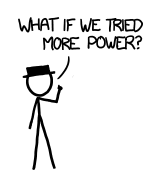
\includegraphics[height=0.3\textheight]{laser_pointer_more_power.png}
  
  \url{https://what-if.xkcd.com/13/}
\end{center}
  
\end{frame}

\begin{frame}{Things are hard if $X_i$ is continuous}
\small
  \begin{itemize}
    \item Clearly, the ``but I controlled for $X$''-regression \texttt{lm(y
    \textasciitilde{} w + x + w * x)} is not consistent (worse still, 
    \texttt{lm(y
    \textasciitilde{} w + x)})
    \begin{itemize}
    \item Not consistent even if $Y,X$ are already demeaned.
      \item \light{Still consistent if we assume complete randomization: $
      (Y
      (1),
                  Y(0)) \indep W$}
    \end{itemize}
    \item Outcome modeling with nonparametric estimator $\hat \mu_w(x)
    \approx \E[Y_i \mid W_i=w, X_i=x]$ and form \[
    \hat\tau_{OM} = \frac{1}{n}\sum_{i=1}^n \hat\mu_1(X_i) - \hat\mu_0
    (X_i) = \frac{1}{n}\sum_{i=1}^n \mu_1(X_i) - \mu_0(X_i) + 
    \text{Approximation Error}
    \]
    would be consistent, but it's tricky to establish normality or
    analytic standard errors.
    \item It is easy
    to see that the approximation error has
    terms like \[
    \frac{1}{n}\sum_{i=1}^n \hat \mu_1(X_i) - \mu_1(X_i) = \overbrace{\E_
    {X}[\hat
        \mu_1(X) - \mu(X)]}^{???} + \overbrace{\pr{\frac{1}{n}\sum_{i=1}^n 
        (\hat \mu_1
    - \mu_1) -
        \E_X(\hat \mu_1 - \mu_1)}}^{\text{hopefully small ($o(1/
        \sqrt{n})$)}}
    \]
    \item The integrated RMSE $\pr{\E_X(\hat \mu_1 - \mu_1)^2}^{1/2}
    \gtrsim n^{-s/(2s+d)} > 1/\sqrt{n}$, so a naive bound would fail
  \end{itemize}
\end{frame}

\begin{frame}{Efficiency of ATE estimators}
\small
  \begin{thm}[Hahn, 1998]
    The semiparametric efficiency bound for the ATE is \[
    V^* = \E\bk{\frac{\sigma_1^2(X_i)}{e(X_i)} + \frac{\sigma_0^2(X_i)}
    {1-e(X_i)} + [\mu_1(X_i) - \mu_0(X_i) - \tau]^2}
    \]
    which is \alert{not} affected by knowledge of the propensity score. 
  \end{thm}
  
  If we \emph{knew} the propensity score, and form the \alert{oracle IPW}
  estimator\[
  \hat\tau_{IPW}^* = \frac{1}{n}\sum_{i=1}^n \frac{W_i Y_i}{e(X_i)} - 
  \frac{(1-W_i)Y_i}{1-e(X_i)}
  \]
  we would find that its variance $V_{IPW}^* > V^*$. 
  
   An easy way to
  remember the the bound is that it is the variance of the oracle 
  \alert{augmented} IPW (AIPW) estimator \[
  \hat\tau^*_{AIPW} = \frac{1}{n}\sum_{i=1}^n \frac{W_i(Y_i-\mu_1(X_i))}{e
  (X_i)} - \frac{(1-W_i)(Y_i-\mu_0(X_i))}{1-e
  (X_i)} + \mu_1(X_i) - \mu_0(X_i)
  \]
  
\end{frame}

\begin{frame}{Efficient estimators}
  \begin{thm}[Imbens, Newey, Ridder (2007); Hahn (1998); Hirano, Imbens,
  Ridder (2003) \ldots]
    Under various tuning parameter choices for estimating $\mu_w, e$ with
    series, the following estimators are first-order equivalent (differ by
    $o_p(1/\sqrt{n})$) and efficient
    \begin{align*}
    \hat\tau_{IPW} &= \frac{1}{n} \sum_{i=1}^n Y_i \pr{\frac{W_i}{\hat e
    (X_i)} - \frac{1-W_i}{1-\hat e(X_i)}} \tag{also self-normalized
    version}\\ 
    \hat\tau_{AIPW} &= \frac{1}{n}\sum_{i=1}^n \pr{\frac{W_i
    (Y_i-\hat \mu_1)}{\hat e
    (X_i)} - \frac{(1-W_i)(Y_i-\hat \mu_0)}{1-\hat e(X_i)}} + \hat\mu_1(X_i) - \hat\mu_0
    (X_i) \\
    \hat\tau_{OM} &= \frac{1}{n} \sum_{i=1}^n \hat\mu_1(X_i) - \hat\mu_0
    (X_i) \\ \hat\tau_{Hahn} &= \frac{1}{n} \sum_{i=1}^n \tilde\mu_1(X_i) - \tilde\mu_0
    (X_i)
    \end{align*}
    where $\tilde \mu_1(X_i) = \frac{\hat\E[Y_iW_i|X=X_i]}{\hat e(X_i)}$
    
  \end{thm}
  
\end{frame}

\begin{frame}{Under the hood}
We can write the ATE problem as a moment problem: \[\E[m(X_i,W_i,Y_i;
\mu_0,\mu_1,e) - \tau] = 0 \quad\text{rewrite to}\quad \E[g(Z_i, \tau, \eta
)] = 0.\]
Our ATE estimates set $\frac{1}{n}\sum_{i=1}^n g(Z_i, \tau, \hat\eta) = 0$.
If we go through the \alert{two-step estimation} argument, we would find
that \[
\hat \tau \simeq \frac{1}{n}\sum_{i=1}^n -G^{-1}\bk{g(Z_i,\beta_0,\eta_0) +
\alert{
\alpha(Z_i)}} = \frac{1}{n}\sum_{i=1}^n \bk{m(X_i,W_i,Y_i;
\mu_0,\mu_1,e) + \alpha(Z_i) - \tau}
\]
where $\alpha(Z_i)$ is an adjustment term that accounts for the first-step
estimation of $\eta$ and $G = \diff{}{\tau}\E[g(Z_i, \tau, \eta_0)] = -1.$

Newey (1994) makes this rigorous.
\end{frame}

\begin{frame}{AIPW / Doubly-robust estimation}
  The AIPW representation is $\tau = \E[\phi(Z)]$ where \begin{align*}
    \phi(Z, \mu_1,\mu_0,e) &= \alert{\mu_1(X) - \mu_0(X)} + \frac{W(Y-\mu_1
    (X))}{e(X)}
  - \frac{(1-W)
  (Y-\mu_0(X))}{1-e(X)} \\ 
  &= \alert{\frac{WY}{e(X)} - \frac{(1-W)Y}{1-e(X)}} - \frac{\mu_1(W-e(X))}
  {e(X)} +
  \frac{\mu_0(W-e(X))}{1-e(X)}
  \end{align*}
  Using the ``wrong'' moment conditions gets an adjustment term  that is
  just right! 
  
  In the IPW case, the adjustment term correlates with the oracle IPW term that
  decreases overall variance
  
  \begin{rmk}[Editorializing]
    People often motivate doubly-robust / AIPW as having two shots at
    getting things right\ldots 
    
    The doubly-robust form is a natural
    representation of the ATE
  \end{rmk}
  
  
\end{frame}

\begin{frame}{A Monte Carlo}

  
  \begin{center}
    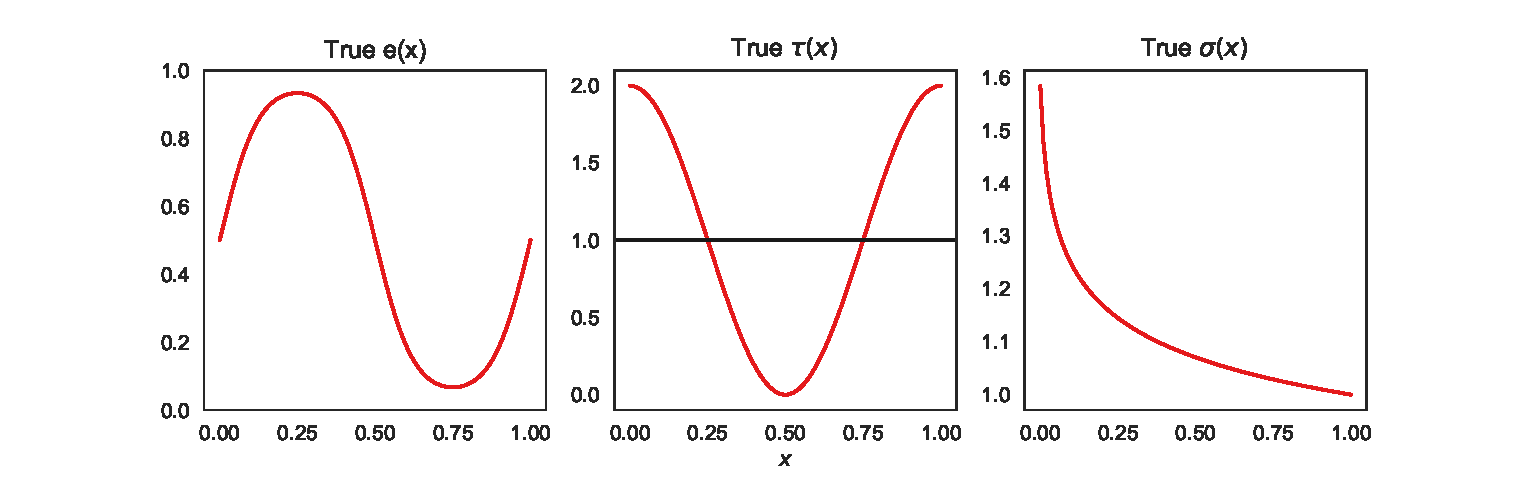
\includegraphics[height=0.5\textheight]{design_simple.eps}
  \end{center}
  
  Scalar $X \sim \Unif$. 
  
  $\E[Y(1)-Y(0)|X] = \tau(X)$. 
  
  $\var(Y(w) | X) =
  \sigma^2(X)$
  
  $\tau = 1$
  
  $e(x) \in [0.05,0.95]$
\end{frame}


\begin{frame}{A Monte Carlo}

  
  \begin{center}
    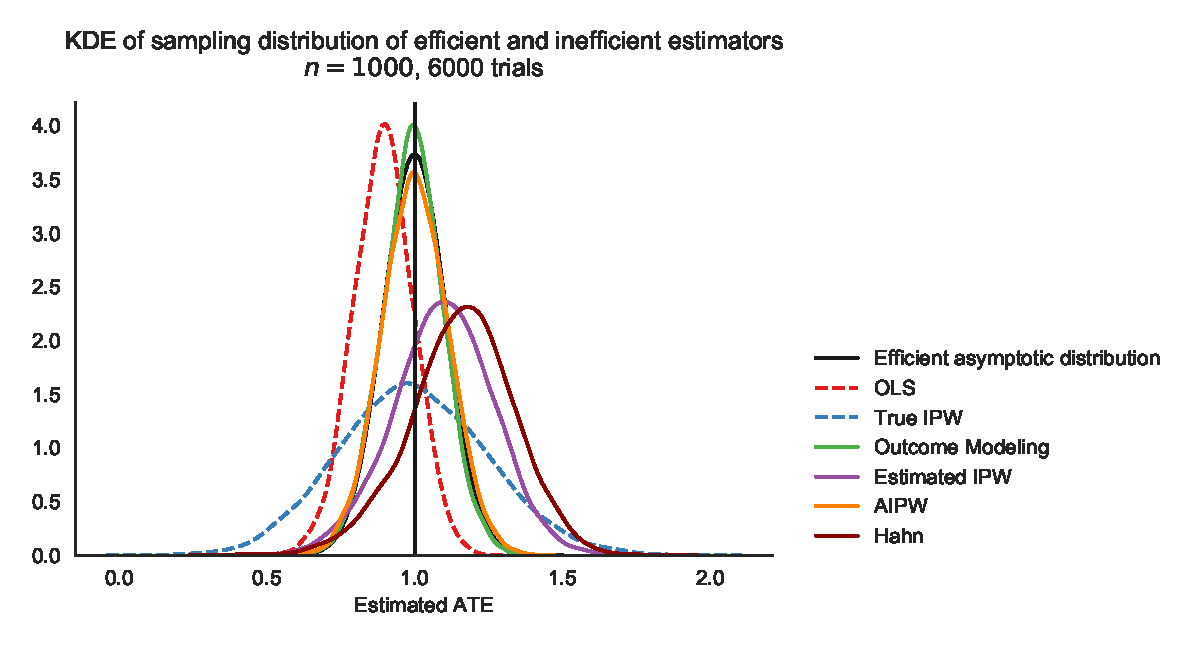
\includegraphics[height=0.8\textheight]{estimators.eps}
  \end{center}
  \scriptsize
  Intuition: OM does better when $\mu_w(x)$ is ``smooth.'' IPW does better
  when $e(x)$ is ``smooth.'' AIPW adapts. 
  
\end{frame}

\begin{frame}{That was not as easy}
  \begin{center}
  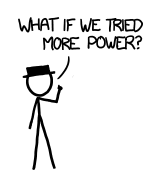
\includegraphics[height=0.3\textheight]{laser_pointer_more_power.png}
  
  \url{https://what-if.xkcd.com/13/}
\end{center}
\end{frame}

\begin{frame}{I promised you machine learning}
  \begin{itemize}
    \item Observation: fitting $\mu_1, \mu_0, e(\cdot)$ are essentially
    prediction problems
    \item Machine learning is \light{(reductively)} a new generation of
    nonparametric estimators that seem to do well in some empirical
    applications
    \item Series estimators perform poorly when $\dim(X) \ge 20$, but
    something like random forest might work quite well
    \item Problem: ML methods are very black box, hard to analyze its
    theoretical properties; classical tools break down
    \item Proposed solution (more-or-less \alert{DML}): Have algorithms
    that work
    relying only on ``weak,''high-level conditions on prediction
    quality \[\text{``$\displaystyle \int (\hat \mu - \mu)^2\,dP(x) = o_p
    (n^
    {-1/4})$''}\]
    Use ``orthogonality'' and sample-splitting to kill terms
    \item \alert{Warning}: overlap  becomes a very strong condition in high
    dimensions
  \end{itemize}
\end{frame}

\begin{frame}[fragile]{DML-AIPW}
\scriptsize
\begin{center}
    \begin{lstlisting}[language=Python]
    data1, data2 = randomly_split_data_in_half(data)
    
    # Train predictor on one half of the data
    mu1_hat_1 = machine_learn("y ~ x", data=data2.where(w == 1))
    mu0_hat_1 = machine_learn("y ~ x", data=data2.where(w == 0))
    e_hat_1 = machine_learn("w ~ x", data=data2)
    
    mu1_hat_2 = machine_learn("y ~ x", data=data1.where(w == 1))
    mu0_hat_2 = machine_learn("y ~ x", data=data1.where(w == 0))
    e_hat_2 = machine_learn("w ~ x", data=data1)
    
    # Compute fitted values on the other half
    e_hat = [e_hat_1(data1), e_hat2(data2)]
    mu1_hat = [mu1_hat_1(data1), mu1_hat_2(data2)]
    mu0_hat = [mu0_hat_1(data1), mu0_hat_2(data2)]
  \end{lstlisting}
\end{center}
  \small
  \[
  \hat \tau_{DMLAIPW} = \frac{1}{n}\sum_{i=1}^n \pr{\frac{W_i
    (Y_i-\hat \mu_{1i})}{\hat e_i} - \frac{(1-W_i)(Y_i-\hat \mu_{0i})}{1-\hat
    e_i}} + \hat\mu_{1i} - \hat\mu_{0i}
  \]
  
\end{frame}

\begin{frame}{Theoretical properties of DML-AIPW}
  \begin{thm}[Stefan Wager's Stat 361; Chernozhukov et al., 2018]
    Let $\hat \tau^*$ be the \alert{oracle AIPW} estimator, which we know
    is efficient. Let $\hat \mu_w, \hat e$ be the machine learning output 
    (which are random). Assume \begin{enumerate}
      \item Overlap 
      \item Uniform consistency \[
      \sup_{x} |\hat \mu_w(x) - \mu_w(x)|,\quad \sup_x|\hat e(x) - e(x)|
      \pto 0
      \]
      \item Risk decay (more-or-less checkable!) \[
      \E\bk{\pr{\hat \mu_w(x) - \mu_w(x)}^2} \E\bk{\pr{\hat e(x) -
      e
      (x)}^2} = o_p(1/n)
      \]
    \end{enumerate}
    Then \[
    \sqrt{n}\pr{\hat\tau_{DMLAIPW} - \hat\tau^*} \pto 0
    \]
  \end{thm}
\end{frame}


\begin{frame}{Monte Carlo, but more power}
  $Y(1), Y(0) \indep W \mid X$, but $X$ can be an image 
  
  \begin{center}
    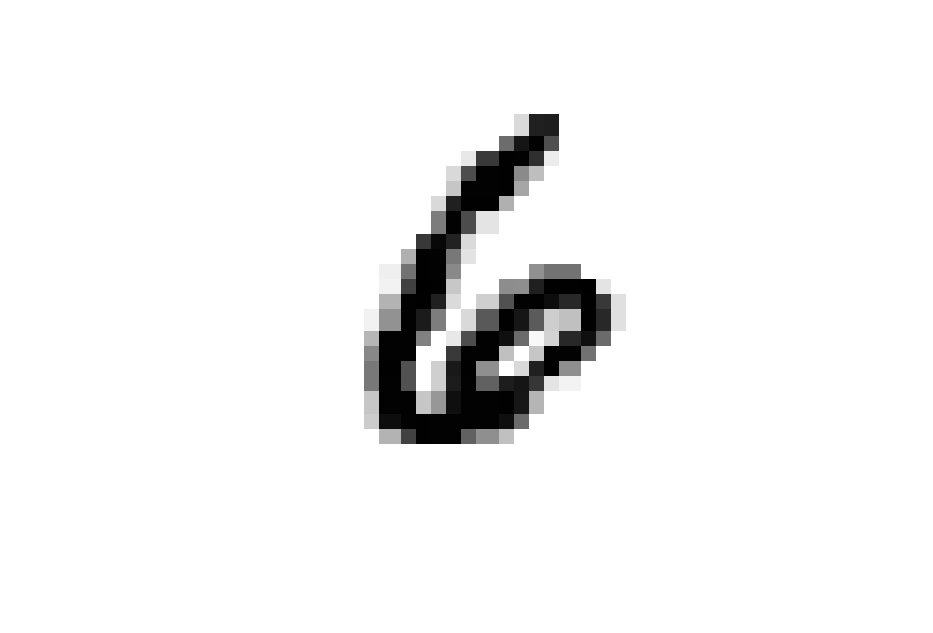
\includegraphics
  [height=20ex]
  {sixmnist.eps}
  
  Represented by $[0,1]^{28 \times 28} = [0,1]^{784}$
  \end{center}
  
  
  Say $e(X) = (\text{digit that $X$ represents}) \times 0.1 + (\text{mean
  pixel
  color})$
  
  Only take $4,5,6$ to make things simple
\end{frame}

\begin{frame}{Ta-da}
  \begin{center}
    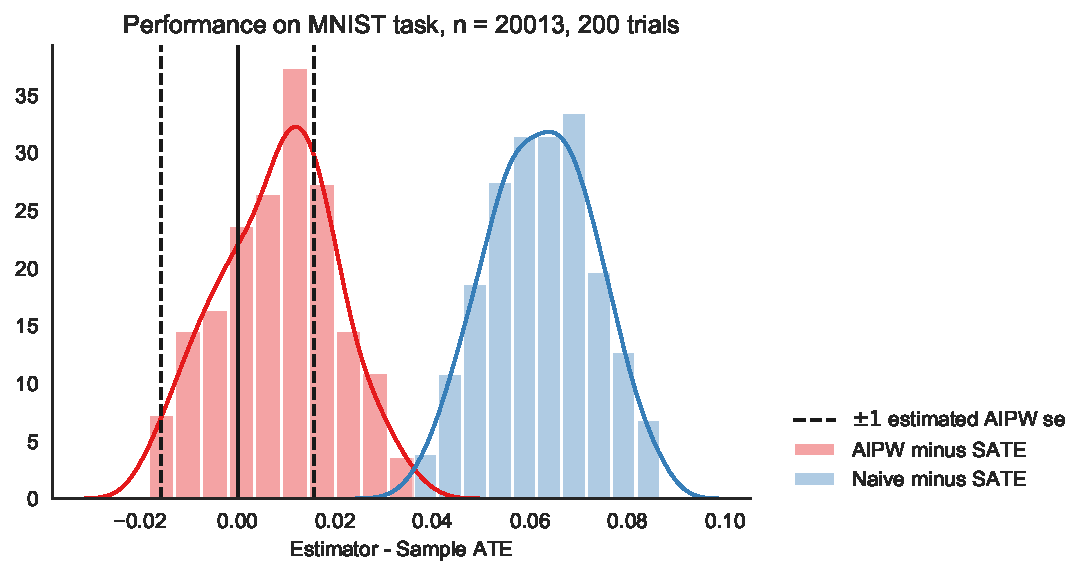
\includegraphics[height=.8\textheight]{mnist.pdf}
  \end{center}
  \scriptsize
  Machine learning via $784 \times 20 \times 1$ ReLU networks + tuning.
  Training takes 3 seconds on my laptop. OLS treating each pixel as a
  covariate is, unsurprisingly, a really bad idea. 
\end{frame}


% \bibliographystyle{ecca}
% \bibliography{../ideas/ref.bib}

\end{document}
